Development of a multi-cellular organism typically starts with a one-cell embryo. This one cell, generated as a result of fertilization (i.e. fusing of the male and female gametes), divides to give rise to the multiple cells and cell types that would eventually form the adult organism. A key question is how the correct arrangement of cells achieved. During development, upto three body axes: anterior-posterior (head-tail), dorsal-ventral (back-front) and left-right, are established. By patterning along these established body axes, proper arrangement of cells can be ensured during development \citep{goldstein1997axis}.

Thus, the body axes serve as the system of spatial axes that allow the embryo to specify position of cells. How are then these body axes established? For many organisms, the embryos start out with few initial asymmetries. Instead, external cues -- such as site of sperm (i.e. male gamete) entry, unequal cell division patterns, and gravity -- are utilized to break the symmetry in the embryo and initiate the establishment of body axes \citep{goldstein1997axis}. Mechanical forces coupled together with chemical patterns translate these external cues into an internal asymmetry of the embryo, by reorganizing certain determinants in the embryo \citep{goldstein1997axis,gross2017active}. As the embryo grows, this unequal distribution of determinants spans across the embryo, thus establishing a body axis \citep{meinhardt2015models,meinhardt2008models}.

It has been observed that the orientation of body axes is relatively fixed with respect to the geometric features of the embryo in many organisms (\autoref{fig:compareBodyAxesEmbryoGeometry}). For example, in many nematodes (roundworms; see \autoref{subfig:compareBodyAxesEmbryoGeometry-apAxisCelegans} for an example in \ac{ce}) the \acl{ap} axis is established at the one-cell stage, and forms along the long axis of the ellipsoidal embryo \citep{goldstein1997axis,goldstein1996specification}. In insect embryos such as fruit flies (see \autoref{subfig:compareBodyAxesEmbryoGeometry-apAxisDrosophila} for an example in \textit{Drosophila}), the \ac{ap} axis forms along the long axis of oocyte \citep{goldstein1997axis,dicko2017geometry,quinlan2016cytoplasmic,shulman2000drosophila,gonzalez1994role}. In chick embryos, Von Baer's rule indicates that the \ac{ap} axis typically forms perpendicular to the long axis of the egg \citep{goldstein1997axis,von1828entwicklungsgeschichte}, but this can be entrained by gravity \citep{kochav1971bilateral}. In mouse embryos (see \autoref{subfig:compareBodyAxesEmbryoGeometry-apAxisMouse}), the \ac{ap} axis initially forms along the axis of the cylindrically-shaped implanted embryo, but then is re-aligned to be along its short axis and transverse to its initial location \citep{tam2004embryonic,vianello2019understanding,hiramatsu2013external,matsuo2017mechanical}. 

\begin{figure}[p]

\centering
\begin{subfigure}{\textwidth}
    \centering
    \includegraphics[width=0.9\textwidth]{Introduction/FigureBodyAxesGeometry/celegans.pdf}
    \caption{\acs{ap} axis in \acs{ce} establishes along the long axis of the ellipsoidal embryo, with posterior half determined by site of sperm entry \citep{goldstein1996specification}. S denotes the sperm at fertilization; AB, P1, ABa, ABp, P2, EMS are names of subsequent blastomeres in embryogenesis (see \autoref{subsec:EarlyEmbryoCelegans} and \cite{strome1989generation}). Top: Sperm enters on the right, away from the female pronucleus -- leading to an embryo with anterior on the left and posterior on the right. Bottom: Sperm enters on the left -- leading to an embryo with anterior on the right and posterior on the left. DV indicates dorso-ventral axis. Adapted from \cite{goldstein1997axis}}
    \label{subfig:compareBodyAxesEmbryoGeometry-apAxisCelegans}
\end{subfigure}
\hfill
\begin{subfigure}{\textwidth}
    \centering
    \includegraphics[width=0.9\textwidth]{Introduction/FigureBodyAxesGeometry/drosophila.pdf}
    \caption{\acs{ap} axis in \textit{Drosophila} is established along the long axis during oogenesis, with posterior half determined by location of oocyte within the germline cyst \citep{gonzalez1994role}. Top: in the usual case, the oocyte migrates towards the posterior of the cyst, specifying the posterior follicle cells that help determine the posterior end. Bottom: if this migration does not occur, no \acs{ap} axis is established. Adapted from \cite{gonzalez1994role}}
    \label{subfig:compareBodyAxesEmbryoGeometry-apAxisDrosophila}
\end{subfigure}
\hfill
\begin{subfigure}{\textwidth}
    \centering
    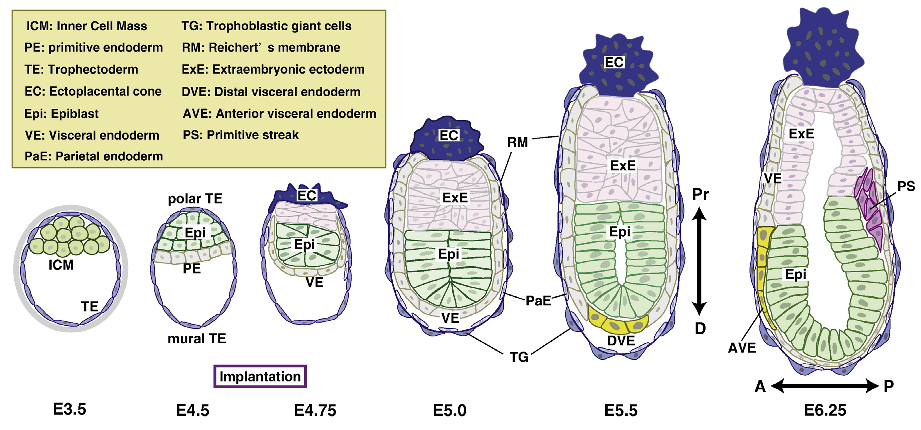
\includegraphics[width=0.9\textwidth]{Introduction/FigureBodyAxesGeometry/mouse.pdf}
    \caption{\acs{ap} axis in mouse is established during uterine implantation. Initial \acs{ap} axis forms along the long axis (Proximal-Distal) of the cylindrical embryo, indicated by the emergence of distal visceral endoderm (DVE) cells at E5.5. \acs{ap} axis reorients to the short axis as the DVE cells migrate to the lateral side, forming anterior visceral endoderm (AVE). Adapted from \cite{matsuo2017mechanical}}
    \label{subfig:compareBodyAxesEmbryoGeometry-apAxisMouse}
\end{subfigure}

\caption[Comparing orientation of \acs{ap} axis with geometry]{Comparing orientation of \acs{ap} axes with embryo geometry in different model organisms: \acs{ce}, \textit{Drosophila}, and mouse}
\label{fig:compareBodyAxesEmbryoGeometry}

\end{figure}

How does this orientation with respect to geometry achieved? Given that mechanical forces are involved in the establishment of body axes, could it be possible that the mechanical forces involved in body axes establishment play a role in achieving this relative orientation? Studies in the mouse embryo seem to suggest so \citep{vianello2019understanding,hiramatsu2013external,matsuo2017mechanical}, but how do mechanical forces enforce this relative orientation is not understood. In this thesis, we will study this problem in the context of \ac{ap} axis establishment in the \ac{ce} embryo - a nematode. We seek to understand the mechanism that ensures that the \ac{ap} axis of the \ac{ce} embryo always establishes along the long axis of the ellipsoidal embryo. 

In this chapter, we first introduce the general features of the cytoskeleton in eukaryotic cells. We will also describe the actomyosin cortex, an important higher-order structure of cytoskeletonal elements present in almost all eukaryotic cells. We then introduce the model organism used in this study: \ac{ce}. We describe the early development of the \ac{ce} embryo. Next, we describe the establishment of \ac{ap} axis in the one-cell stage \ac{ce} embryo. We also introduce the phenomenon of \ac{ap} axis alignment -- the active reorientation of the \ac{ap} axis such that it aligns with the geometric long axis of the ellipsoidal embryo. Finally, we provide an overview of the thesis, encapsulating our work on elucidating the mechanism of \ac{ap} axis alignment in \ac{ce} embryo.

\section{Cytoskeleton}\label{sec:Cytoskeleton}
As noted above, mechanics plays an important role in the establishment of body axes. Cells thus need to react to the mechanics of their surrounding, and modify their own mechanical properties in response to different stimuli. The structure that allows cells to actively modify their mechanical properties, and perform mechanical tasks, is the cytoskeleton \citep{chaffey2003alberts,bray2001cell,fletcher2010cell}. It is essential in many cellular processes: maintaining cell shape \citep{chaffey2003alberts,rivero1996role,herrmann2007intermediate}, driving locomotion \citep{fletcher2010cell}, and cell division \citep{chaffey2003alberts,gonczy2001spindle}. Its role is to provide the cell with a dynamic mechanical scaffolding, allowing the cell to act as a highly adaptive mechanical entity to achieve different tasks \citep{chaffey2003alberts,bray2001cell,fletcher2010cell}.

The cytoskeleton is commonly defined as a network of protein filaments that extend throughout the cytoplasm of eukaryotic cells, although analogous filaments have also been identified in prokaryotes \citep{erickson2007evolution}. This meshwork of filaments is complemented by motor proteins that exert force betwen the filaments, crosslinking proteins that tie these filaments in the meshwork and various associated proteins that modify and remodel the meshwork \citep{chaffey2003alberts,bray2001cell,fletcher2010cell}. In this section, we will introduce these elements that make the cytoskeleton in eukaryotic cells. We will also introduce the actomyosin cortex, a thin layer of cytoskeletonal elements present just below the cell membrane \citep{chaffey2003alberts,salbreux2012actin}, and the primary force-generating mechanical structure that this work focuses on.

\subsection{Main constituents of the cytoskeleton}\label{subsec:ComponentsCytoskeleton}
\subsubsection{Protein Filaments}\label{subsubsec:FilamentsCytoskeleton}
Protein filaments provide the backbone of the cytoskeleton. In eukaryotic cells, the cytoskeleton is composed of three principal types of protein filaments: actin filaments, intermediate filaments and microtubules. Monomeric protein subunits build each of these filaments. In contrast to usual polymers, these filaments are held together by non-covalent bonds, allowing fast assembly and disassembly \citep{chaffey2003alberts}. 

\paragraph{Actin filaments}
Actin filaments (or F-actin) are right-handed double helix composed of two protofilaments, each being a chain of actin monomers (or G-actin) \citep{pollard1986actin,pollard2000molecular} (see \autoref{subfig:cytoskeletonMainConsituents-actin}). Actin filaments are thin, with a typical diameter of around \SI{7}{\nano\meter} \citep{cooper2007cell}, and flexible, with a typical persistence length of \SI{17}{\micro\meter} \citep{ott1993measurement,gittes1993flexural}. The pitch of the helix formed by the protofilaments is typically around \SI{37}{\nano\meter}. Polymerisation of actin filaments is fueled by hydrolysis of \ac{atp} at the binding site on the monomers as they bind to the filament \citep{fujiwara2007polymerization}. Actin filaments are structurally polar, with a defined (+) or barbed end where new monomers preferentially bind, and a (-) or pointed end where monomers preferentially unbind \citep{pollard1986actin,pollard2000molecular,vavylonis2005actin}. Thus, actin filaments can undergo tread-milling, regulated by \ac{atp} \citep{wegner1982treadmilling}.

Actin filaments often gets organized into higher-order structure, such as the actomyosin cortex (which we describe below), to perform various functions such as migration \citep{pollard2003cellular}, cell division \citep{sanger1975changing} and control of cell shape \citep{clarke1977nonmuscle}. 

\paragraph{Microtubules}
Microtubules are rigid hollow rod-like polymers, formed by the polymerization of a dimer of two globular proteins, $\alpha$-tubulin and $\beta$-tubulin \citep{chaffey2003alberts,nogales1998structure} (see \autoref{subfig:cytoskeletonMainConsituents-microtubule}). These dimers polymerize to form linear protofilaments that associate laterally to form the microtubule \citep{chaffey2003alberts}. Slight offset between protofilaments generates a pseudo-helical structure \citep{hunyadi2007microtubule}. The typical \enquote{\num{13}-\num{3}} arrangement, composed of \num{13} protofilaments with \num{3} dimer offset between neighbouring pairs, has a diameter of approximately \SI{25}{\nano\meter}, and a persistence length of approx \SI{5}{\milli\meter} \citep{chalfie1979organization,chaffey2003alberts,gittes1993flexural,ledbetter1963microtubule} -- practically rigid in most cells, given their typical sizes. Similar to actin filaments, microtubules are also polar, with a fast growing (+) end and a slow growing (-) end \citep{howard2003dynamics}. Microtubules serve various functions such as providing mechanical support, facilitating cell migration and locomotion \citep{mikhailov1998relationship}, acting as pathways for intracellular transport \citep{chaffey2003alberts}, and centering of the mitotic spindle \citep{pearson2004dynamic,grill2003distribution,grill2005theory}.

\textit{Centrosome}: Microtubules usually are nucleated at, and extend outwards from, a \ac{mtoc}, to which the (-) ends are attached. In animal cells, the major \ac{mtoc} is the centrosome, typically present near the nucleus when the cell is not dividing. At mitosis (i.e. when the cell is dividing), the centrosome duplicates \citep{chaffey2003alberts}. In most animal cells, a centrosome consists of a pair of cylinders (centrioles) surrounded by a meshwork of pericentriolar material \citep{pimenta2020pericentriolar}. Complexes of $\gamma$-tubulin in the centrosome serve as the nucleation sites for microtubule assembly \citep{kellogg1994centrosome}. In many animals, centrosomes play an important role in the formation of the mitotic spindle, an array of microtubules and associated proteins responsible for proper segregation of genetic material in the daughter cells after division \citep{bettencourt2013q,chaffey2003alberts}.

\paragraph{Intermediate filaments}
Different cell types also produce other filaments, with a typical diameter of \SI{10}{\nano\meter}. They typically play a structural role and provide mechanical support \citep{chaffey2003alberts,herrmann2007intermediate}.

\subsubsection{Motor proteins}\label{subsubsec:MotorCytoskeleton}
Motor proteins convert the chemical energy released in \ac{atp} hydrolysis into mechanical work \citep{chaffey2003alberts,bray2001cell,kolomeisky2007molecular,howard2002mechanics}. Motor proteins are categorized into three super-families, distinguished by the type of filaments they bind to. \textit{Myosins} are motors associated with actin filaments, while \textit{kinesins} and \textit{dyenins} bind to microtubules instead \citep{chaffey2003alberts}. Molecular motors perform various functions \citep{chaffey2003alberts}, such as cargo transport \citep{vale2003molecular} and serving as force generators for contraction of large-scale structures \citep{howard2002mechanics,carlsson2006contractile}.

Generally, motor proteins share a common set of \enquote{mechanical parts}: a track on which the motor walks (typically the protein filaments), some fuel (typically \ac{atp}), a transducer and force generator that converts the chemical energy of the fuel into a \enquote{power stroke} to generate mechanical force and a lever that transmits that force to the track \citep{hwang2009mechanical}. We illustrate this using the example of a particular myosin - \acs{nmy2}, which is a major component of the actomyosin cortex. 

\paragraph{\acl{nmy2}}
\ac{nmy2} is a member of the myosin super-family of motor proteins, and therefore a molecular motor that acts on actin filaments (see \autoref{subfig:cytoskeletonMainConsituents-myosin}). It is a major contractile protein of non-muscle eukaryotic cells \citep{chaffey2003alberts,holmes2008myosin}. \ac{nmy2} forms a hexamer consisting of three pairs of polypeptides: two heavy chains, two regulatory light chains involved in regulation of \ac{nmy2} activity and two essential light chains which stabilize the heavy chain conformation \citep{holmes2008myosin,vicente2009non}. Each heavy chain has a motor domain on one end (N-terminus) that binds to actin filament and \ac{atp}, followed by a neck domain to which the regulatory light chains bind, and a coiled-coil domain on the other end (C-terminus) that facilitates dimerization of the heavy chain \citep{holmes2008myosin,vicente2009non,robert2019force}. \ac{nmy2} usually organizes into myosin minifilaments, consists of around \num{28} \ac{nmy2} units \citep{holmes2008myosin,vicente2009non}. 

How does the \ac{nmy2} motor generate force? When not bound to \ac{atp}, myosin has a strong affinity to actin filament. \ac{atp} binding leads to dissociation of the motor domain from the actin filaments, and \ac{atp} hydrolysis ensues. During this step, the neck domain bends, allowing the motor domain to sample sites on the actin filaments. As myosin binds again to the filament, the products of \ac{atp} hydrolysis are released, resulting in the force generating step (that is, the power stroke) that displaces the motor along the filament with \SI{5}{\nano\meter} displacement, and returns it back to the initial state \citep{de2004relating,sweeney2010structural,tyska2002myosin,robert2019force}. We refer the reader to \autoref{subfig:cytoskeletonMainConsituents-powerstroke} for a depiction of the power stroke of myosin. Thus, the motor domains act as the transducer and force generators, the neck domain as the lever, the actin filament as the track and \ac{atp} as fuel for the \ac{nmy2} motor \citep{robert2019force,hwang2009mechanical}. \ac{nmy2} is a non-processive motor (it only makes one step before it detaches from the track \citep{howard2002mechanics,hwang2009mechanical}) with a low duty cycle (fraction of time spent bound to actin filament \citep{howard2002mechanics,hwang2009mechanical}) \citep{kovacs2003functional,wang2003kinetic}. Minifilaments of \ac{nmy2} can slide actin filaments past each other, by creating force dipoles \citep{vicente2009non,niederman1975human,mahajan1996assembly}. \ac{nmy2} also serves as an actin crosslinker \citep{xu2001during,mizuno2007nonequilibrium,laevsky2003cross}.

\begin{figure}[p]

\centering
\begin{subfigure}{\textwidth}
    \centering
    \includegraphics[width=0.9\textwidth]{Introduction/FigureCytoskeleton/actin.pdf}
    \caption{Sketch of an actin filament, red circles denote monomeric G-actin. Arrows indicate rate of chemical reaction at each end. Adapted from \cite{sebastian2012activeChiral}}
    \label{subfig:cytoskeletonMainConsituents-actin}
\end{subfigure}
\hfill
\begin{subfigure}{\textwidth}
    \centering
    \includegraphics[width=0.9\textwidth]{Introduction/FigureCytoskeleton/microtubules.pdf}
    \caption{Sketch of a \enquote{13-3} microtubule, composed of $\alpha$ and $\beta$ tubules. Arrows indicate rate of chemical reaction at each end. Adapted from \cite{sebastian2012activeChiral}}
    \label{subfig:cytoskeletonMainConsituents-microtubule}
\end{subfigure}
\hfill
\begin{subfigure}{\textwidth}
    \centering
    \includegraphics[width=0.9\textwidth]{Introduction/FigureCytoskeleton/myosin.pdf}
    \caption{Schematic of the forms of \acs{nmy2} motor protein. i) \acs{nmy2} converts from inactive state (left) to active state (right) via phosphorylation. Active state has three domains: the globular head containing the motor and actin binding domains, the neck domain or lever arm, and a long coiled-coil domain of heavy chains. ii) \acs{nmy2} can assemble into bipolar filaments -- myosin minifilaments -- and can slide antiparallel actin filaments past each other. Adapted from \cite{vicente2009non}}
    \label{subfig:cytoskeletonMainConsituents-myosin}
\end{subfigure}
\hfill
\begin{subfigure}{\textwidth}
    \centering
    \includegraphics[width=0.85\textwidth]{Introduction/FigureCytoskeleton/powerstroke.pdf}
    \caption{Schematic of the power stroke of \acs{nmy2}. Refer to text for details on power stroke. Adapted from \cite{de2004relating}}
    \label{subfig:cytoskeletonMainConsituents-powerstroke}
\end{subfigure}

\caption[Main constituents of the cytoskeleton]{Main constituents of the cytoskeleton in eukaryotic cells}
\label{fig:cytoskeletonMainConsituents}

\end{figure}

\subsubsection{Associated proteins}\label{subsubsec:AssociatedProteinsCytoskeleton}
Most of the known cytoskeletal proteins are neither filamentenous nor motors. Instead, they modify and interact with the existing protein filaments and motors, to dynamically alter the mechanical properties of the cytoskeleton. We refer the reader to \cite{chaffey2003alberts,pollard1986actin} for a comprehensive overview of these proteins and their functions; here, we will briefly review some of the important functions these proteins fulfill.

\textit{Nucleators} help initiate the formation of protein filaments, by providing a nucleation point. \textit{Capping proteins} bind to the ends of filaments, blocking polymerisation at the end where they bind. These proteins thus can either stabilise or de-stabilise a protein filament, depending on where they bind. \textit{Severing proteins} cut filaments. \textit{Crosslinkers} and \textit{bundling proteins} organize protein filaments into structured networks, and modify them. \textit{Sequestering proteins} help with recycling unbound monomers, while \textit{Sidebinding proteins} act as molecular rulers. \textit{Linkers} link filaments of different kinds, allowing different filaments (such as the microtubules and actin filaments) to influence each other. \textit{Regulators} regulate the action of other proteins. Note that individual proteins can have multiple functions, and thus belong to multiple categories.

\subsection{Actomyosin cortex}\label{subsec:ActomyosinCortex}

\begin{figure}[h]
    \centering
    \includegraphics[width=\textwidth]{Introduction/FigureActomyosin/actomyosinSketch.pdf}
    \caption[Sketch of actomyosin cortex]{Sketch of the actomyosin cortex as a quasi-2D polymeric meshwork of actin filaments below the cell membrane (composed of lipids) and interspersed with myosin motors and other proteins. Top represents an effective 2D representation of the actomyosin cortex that could be obtained by averaging over the thickness of the cortex. Adapted from \cite{kumar2021actomyosin}}
    \label{fig:actomyosinCortexSketch}
\end{figure}

The actomyosin cortex, also called the cell cortex, is a thin (around few hundred nanometers \citep{clark2013monitoring}) polymeric meshwork of cross-linked actin filaments, interspersed with myosin motors and associated proteins, that lies just below the cell membrane of most eukaryotic cells \citep{bray1988cortical,chaffey2003alberts} (see \autoref{fig:actomyosinCortexSketch}). Analysis using cryo-electron tomography and atomic force microscopy revealed that actin filaments organize in both isotropic meshworks and actin bundles \citep{hartwig1991cytoskeleton,heuser1980filament,morone2006three,medalia2002macromolecular,pesen2005micromechanical}. 

The cortex is not, however, a static structure -- \ac{atp} hydrolysis fuels the polymerization and de-polymerization of actin filaments, activity of the associated proteins, and force generation by myosin motors. This external energy input and resultant active remodeling of the cortex drives it far from equilibrium, and makes it a very dynamic structure. This highly cross-linked and dynamic nature of the cortex makes it behave like a viscoelastic material \citep{kumar2021actomyosin,salbreux2012actin}, as confirmed by laser ablation experiments \citep{saha2016determining,mayer2010anisotropies}. In live cells, the active remodeling in the cortex occurs on timescales of around \SI{30}{\second} \citep{fritzsche2016actin}, and elastic stresses relax on comparable timescales \citep{saha2016determining}. As a consequence, the cortex can effectively be considered as a viscous fluid on longer timescales. Force generation by myosin motors confer the cortex with a tendency to actively contract \citep{carlsson2006contractile} -- the actomyosin cortex can thus be considered as active viscous fluid. In \autoref{ch:ActiveMatter}, we will discuss the behaviour of actomyosin cortex as an active fluid in the context of the \ac{ce} cortex during \ac{ap} axis establishment.

Actomyosin cortex helps the cell to adapt to changing environmental conditions by controlling cell mechanics. The cortex determines the stiffness of the cell surface, and opposes osmotic pressure \citep{stewart2011hydrostatic}. Global increase in contractility of the cortex facilitates the rounding of the cell before its division \citep{kunda2008moesin}. Local changes in cortex contractility can create gradients of cortical tension. Such changes can aid in cell migration, via retraction of the rear of the cell from the substrate \citep{vicente2009non}. Developmental processes at the tissue scale can also be directed by the cortex of the constituent cells \citep{rauzi2011cortical} -- such as dorsal closure in \textit{Drosophila} \citep{martin2010pulsation} and convergence extension in \textit{Xenopus} \citep{zhou2009actomyosin}. In \autoref{sec:ApAxisEstablishment}, we will discuss how the local changes in contractility in the one-cell stage \ac{ce} embryo drive flows in the cortex, and what role these cortical flows play in the \ac{ap} axis establishment of \ac{ce} \citep{mayer2010anisotropies}.

\section{\acs{ce} as a model organism}\label{sec:CelegansModel}

\begin{figure}[h]
    \centering
    \includegraphics{Introduction/FigureWorm/worm.pdf}
    \caption[\acs{ce} worm and one-cell embryo]{Microscope picture of \acs{ce} worm (top) and one-cell stage embryo (bottom), by M. Leaver (used with permission). A and P mark the anterior and posterior of the developing embryo. Typical location of the one-cell embryo in the gonad of the worm, and its length (approx. \SI{50}{\micro\meter}) is marked}
    \label{fig:celegansWormModelOrganism}
\end{figure}

\ac{ce} was first considered as a potential model organism by Sydney Brenner over 50 years ago. After witnessing the importance of the T4 bacteriophages as the ideal 'model organisms' for research in molecular biology, he searched for a model organism to replicate the same successes in developmental biology and neuroscience \citep{wb1988nematode,brenner1974genetics,brenner2003nature}. He found his model organism of choice in the small nematode \ac{ce}, a self-fertilizing hermaphrodite with rare spontaneous males (less than \num{0.2}\% of worms \citep{haag2005evolution,corsi2015transparent}) \citep{brenner1974genetics}. Today, there are more than thousand research groups that use \ac{ce} as a model organism, due to the above ease of maintenance and the multitude of biological tools available for study and manipulation of \ac{ce} worms, in various fields such as neuroscience, development, ecology and cell biology \citep{corsi2015transparent}.

\ac{ce} is a free-living transparent nematode, typically found in temperate climate around the world. It feeds on bacteria, typically \ac{ecoli} on the surface of agarose plates when cultured in lab \citep{brenner1974genetics}. In lab conditions, \ac{ce} worms grow from initial larval stage (\SI{0.25}{\milli\meter} long) to final adult stage (\SI{1}{\milli\meter} long) in around \num{3} days at \SI{20}{\celsius}, although this time can vary with temperature and food available \citep{corsi2015transparent,brenner1974genetics,lee2009regulation}. It is a simple organism in both anatomy and genome. It has a fixed, genetically determined, number of cells at the adult stage, with adult hermaphrodite at 959 somatic cells and adult male at 1033 cells \citep{sulston1983embryonic,kimble1979postembryonic}. One of most prominent features of \ac{ce} is its invariant cell lineage: every worm follows the same pattern of cell divisions and results in the same number of cells, i.e. the developmental fate of every somatic cell is invariant. This has enabled tracing the fate of cell during development, giving rise to a complete map of cell lineage \citep{sulston1983embryonic,sulston1975dopaminergic,kimble1979postembryonic}. 

Hermaphrodites and males differ in their adult morphology, with males being a bit thinner and shorter, and possess a distinctive tail \citep{corsi2015transparent}. The primary method of reproduction in \ac{ce} is via self-fertilization: hermaphrodites produce both sperms and oocytes, which fertilize each other. A hermaphrodite typically lays about 300 eggs. Males can also fertilize the hermaphrodites, allowing for a form of sexual reproduction. The young worms hatch and subsequently go through four larval stages (L1-L4) before adulthood. These adults are fertile for about \num{3} days, and have an average lifespan of about \numrange{2}{3} weeks \citep{corsi2015transparent}. In harsh conditions, larval development can be paused -- these worms can survive several months in a special state called dauer arrest \citep{hu2007dauer}.

The above properties of \ac{ce} make it very convenient to use as a model organism for development \citep{corsi2015transparent,brenner1974genetics}. It is easy to maintain and grow in bulk due to the large number of progeny and rapid life cycle. Worms can be easily frozen for years and revived later when needed. Individual worms can be easily observed at the level of single cells under the microscope due to their transparency. Its small size allows complete anatomical description even at the electron microscope level. Self-fertilization means a single worm can generate an entire population of its clones, while the rare males, which can be maintained, enable transfer of genetic markers between populations. \ac{ce} is also the first multi-cellular organism with a completely sequenced genome, containing about 18000 predicted genes \citep{c1998genome}. Together with the simple feeding method of double stranded \ac{rnai} in \ac{ce} \citep{kamath2003genome}, all these properties of \ac{ce} make genetic perturbations in \ac{ce} worms a simple and efficient process. Using fluorescent proteins such as \ac{gfp} to tag the proteins in the embryo allows in-depth study of its development \citep{chalfie1994green,boulin2006reporter}.

\subsection{Early embryogenesis in \acs{ce}}\label{subsec:EarlyEmbryoCelegans}

\begin{figure}

\centering
\begin{subfigure}{\textwidth}
    \centering
    \includegraphics[width=\textwidth]{Introduction/FigureEarlyEmbryogenesis/firstCellEvents.pdf}
    \caption{Chronological sequence of events in the one-cell stage embryo, from fertilization until the first cell division. See \autoref{subsec:EarlyEmbryoCelegans} and \autoref{subsec:mechanismApAxisEstablishment} for further details. Anterior is to the left, posterior to the right. Grey circles represent pronuclei and nuclei, black circle extruded polar bodies, purple circle centrosomes. Microtubules are denoted in light grey, arrows illustrate movement. Blue represents \acs{ppar}, red represents \acs{apar}. Adapted from \cite{mirjam2010mechanics}. Also see \cite{schneider2003cell}.}
    \label{subfig:embryogenesisCelegans-onecell}
\end{subfigure}
\hfill
\begin{subfigure}{\textwidth}
    \centering
    \includegraphics[width=\textwidth]{Introduction/FigureEarlyEmbryogenesis/fullEmbryogenesis.pdf}
    \caption{Sketch depicting early embryogenesis in \acs{ce} embryo. The one-cell stage embryo, after fertilization, undergoes an asymmetric division, forming the larger, anterior AB cell and smaller, posterior P1 cell. AB gives rise to somatic cells only. P1 divides further, generating somatic blastomeres EMS (which divides into E and MS), C and D, and the germline progenitor P4. Tissues that the blastomeres give rise to are indicated next to them. Adapted from \cite{mirjam2010mechanics}. Also see \cite{strome1989generation}.}
    \label{subfig:embryogenesisCelegans-full}
\end{subfigure}

\caption[Early embryogenesis in \acs{ce}]{Early embryogenesis in \acs{ce} embryo}
\label{fig:embryogenesisCelegans}

\end{figure}

\ac{ce} embryogenesis begins when a mature oocyte, arrested in meiosis I, is fertilized by a sperm \citep{rose2014polarity,begasse2011} -- see \autoref{subfig:embryogenesisCelegans-onecell}. As we will discuss later on, the site of sperm entry defines the future posterior end of the embryo \citep{goldstein1996specification} (also, see \autoref{subfig:compareBodyAxesEmbryoGeometry-apAxisCelegans}). Prior to fertilization, the oocyte is fairly symmetric \citep{cuenca2003polarization,cowan2004asymmetric,schonegg2006cdc}. Thus, sperm entry represents the first event in which symmetry is broken in the oocyte. At fertilization, the sperm donates its genetic material -- the male pronucleus -- to the embryo, along with centrosomes \citep{o2000spd,wallenfang2000polarization,cowan2004centrosomes}. After fertilization, meiosis is completed with the extrusion of two polar bodies, usually located at the anterior end. A rigid ovoid-shaped chitin eggshell is secreted by the newly formed embryo after fertilization -- which provides the embryo with its ellipsoidal shape \citep{johnston2012eggshell}.

Events in the one-cell stage of the \ac{ce} embryo -- called the P0 stage -- can be divided into two phases: establishment phase and maintenance phase \citep{cuenca2003polarization}. Establishment phase is initiated by the centrosomes near the male pronucleus. These centrosomes organize microtubule asters, which lead to triggering the establishment of the \ac{ap} axis (discussed below). In the establishment phase, large-scale flows in the actomyosin cortex (directed away from the male pronucleus) and cytoplasm (directed towards the male pronucleus) are observed, which gives the establishment phase its other name -- flow phase. Towards the end of establishment phase, the female pronucleus migrates towards and meets with the male pronucleus, concomitant with a characteristic constriction at the mid of the embryo -- called the pseudocleavage furrow \citep{cuenca2003polarization,nigon1960architecture,reymann2016cortical}. This migration is powered by the microtubules connecting the two pronuclei late in the establishment phase \citep{niwayama2011hydrodynamic}. Pronuclear meeting indicates the end of establishment phase and start of the maintenance phase.

In the maintenance phase, the \ac{ap} axis orientation is maintained -- no flows in the actomyosin cortex or cytoplasm are observed. P granules, which play a role in determining germline fate, localize towards the posterior end, as dictated by the established \ac{ap} axis \citep{gonczy2008mechanisms,hoege2013principles}. The mitotic spindle is set up in the center of the embryo, but elongates towards the posterior end following pronucleus envelope breakdown \citep{grill2003distribution}. The spindle is observed to rock, i.e. oscillate \citep{grill2005theory}. Towards the end of maintenance phase, the P0 cell divides asymmetrically (due to the eccentric location of the mitotic spindle). This results in a large cell towards the anterior and a smaller cell at the posterior, termed AB and P1 respectively. 

These cells divide further as the embryo develops, as depicted in \autoref{subfig:embryogenesisCelegans-full}. The established AP axis is however retained by the distribution of P granules as the embryo develops, as the P granules segregate into the germline precursor cells: P1, P2, P3, P4 \citep{rose2014polarity,strome1989generation}. The P4 cell is the primodial germ cell -- all sperms and oocytes generated in the new worm originate from this P4 cell \citep{rose2014polarity,kimble2005germline}.

\section{\acs{ap} axis establishment in \acs{ce}}\label{sec:ApAxisEstablishment}
In this section, we will discuss in detail the mechanism of \ac{ap} axis establishment in \ac{ce}. As noted above, the \ac{ap} axis is established during the establishment phase at the one-cell stage during \ac{ce} embryogenesis \citep{rose2014polarity}. \ac{ap} axis is established via a cell polarization event mediated by \acs{par} polarity proteins \citep{motegi2013network,hoege2013principles,lang2017proteins}. In this section, we will first discuss the \acs{par} polarity system -- a conserved system of proteins involved in cell polarization in many eukaryotic cells \citep{hoege2013principles}. Next, we will discuss the \ac{ap} axis establishment process, detailing the role of the actomyosin cortex and the centrosomal trigger from the male pronucleus. Finally, we will introduce the phenomenon this work is mainly concerned with: \ac{ap} axis alignment. We will also discuss the proposed mechanisms for \ac{ap} axis alignment.

\subsection{\acs{par} polarity system}\label{subsec:ParPolarity}
\ac{par} proteins are a conserved set of proteins in eukaryotes, functioning to control asymmetric cell division and partitioning of components in many cell types \citep{goldstein2007proteins,knoblich2001asymmetric}, and crucial in cell polarity establishment \citep{goldstein2007proteins}. \ac{par} proteins were first identified in the \ac{ce} embryos, as a result of genetic mutations that cause symmetric division of the one-cell embryo \citep{guo1995par1,kemphues1988identification}. 

As noted above, \ac{par} proteins help establish the \ac{ap} axis in \ac{ce} via polarization of the one-cell stage embryo. \ac{par} proteins can be classified into three groups based on their localization in this polarized embryo: PAR-4 and PAR-5 remain uniformly distributed on the cortex, PAR-1, PAR-2, LGL-1 (\ac{ppar}) localize to the posterior half of the cortex and PAR-3, PAR-6, PKC-3 (\ac{apar}) localize to the anterior half of the cortex \citep{motegi2013network}. Importantly, this localization is specific to the cortex (but not absolute) - \ac{par} proteins are uniformly distributed in the cytoplasm \citep{motegi2013network,hoege2013principles}. 

Experiments using Fluorescent recovery after photo-bleaching and fluorescent correlation spectroscopy have revealed that \ac{par} proteins can exchange between the cortex and the cytoplasm, and also diffuse laterally on the cortex \citep{hoege2013principles,goehring2011proteins,schubert2000mex,petravsek2008characterization}. Extensive mixing between the \ac{apar} and \ac{ppar} on the cortex is prevented by the mutual inhibition between the two groups: \ac{apar} inhibit the binding of \ac{ppar} to the cortex occupied by \ac{apar}, and vice versa \citep{hoege2013principles,motegi2013network}. The behaviour of \ac{par} proteins on the cortex can be modelled as a reaction-diffusion system, with characteristics similar to those observed \emph{in vivo} \citep{hoege2013principles}. Importantly, \ac{par} proteins can interact with the actomyosin cortex -- \ac{apar} can reduce the dissociation rate of \ac{nmy2} from the cortex \citep{gross2019guiding}, while flows in the cortex can advect the \ac{par} proteins \citep{goehring2011advectionpolarization}. 

\subsection{Mechanism of \acs{ap} axis establishment}\label{subsec:mechanismApAxisEstablishment}

\begin{figure}

\centering
\begin{subfigure}{\textwidth}
    \centering
    \includegraphics[width=\textwidth]{Introduction/FigureApAxisEstablishment/ApAxisEstablishmentEvents.pdf}
    \caption{Schematics depicting the major events that occur in \acs{ap} axis establishment in one-cell \acs{ce} embryo. i) Polarity trigger is provided by the centrosome towards the future posterior end of the embryo, via microtubules and other diffusive components \citep{hoege2013principles}. This trigger displaces the \acs{apar} and down-regulate the actomyosin cortex near the trigger \citep{hoege2013principles,gross2019guiding}. ii) View onto the cell Cortex during \acs{ap} axis establishment. Actomyosin cortex is less cross-linked and less dense in the posterior domain (indicated by \acs{ppar}) compared to anterior domain (indicated by \acs{apar}). The cortex also shows anisotropic tension \citep{mayer2010anisotropies}, with cortical flow directed towards the anterior. Flow speeds are larger in the posterior compared to anterior. iii) Cross-section of the cell cortex. Cortical flows passively transport the \acs{par} proteins by advection \citep{goehring2011advectionpolarization}. Adapted from \cite{hoege2013principles}} 
    \label{subfig:apAxisEstablishmentMechanism-schematics}
\end{subfigure}
\hfill
\begin{subfigure}{\textwidth}
    \centering
    \includegraphics[width=\textwidth]{Introduction/FigureApAxisEstablishment/ApAxisEstablishmentCortexMicrograph.pdf}
    \caption{Cortical activity during \acs{ap} axis establishment. Top: DIC images taken in the midplane of the embryo. Bottom: \acs{nmy2}::\acs{gfp} images taken at the surface of the embryo; that is, in the cortical plane. Anterior is to the left, posterior to the right. $T=$ \SI{0}{\second} indicates start of establishment phase, with myosin forming foci-like structures uniformly in the cortex. After polarization is triggered near the male pronucleus, anterior-directed cortical flows cause the cortex to retrace from the posterior end (ex: $T=$ \SI{225}{\second}). The cortex completely retracts by the time the pseudocleavage furrow forms ($T=$ \SI{495}{\second}), and the two domains have formed. Establishment phase ends at pronuclear meeting ($T=$ \SI{705}{\second}), with myosin foci disappearing from the cortex. Yellow arrows indicate pronuclei (female on the left, male on the right) and blue arrows represent the ingression formed by the pseudocleavage furrow. Scale: \SI{10}{\micro\meter}. Adapted from \cite{sundar2012regulation}}
    \label{subfig:apAxisEstablishmentMechanism-micrograph}
\end{subfigure}

\caption[\acs{ap} axis establishment in \acs{ce}]{Mechanism of \acs{ap} axis establishment in one-cell stage \acs{ce} embryo}
\label{fig:apAxisEstablishmentMechanism}

\end{figure}

\ac{ap} axis establishment starts around \SI{30}{\minute} after fertilization, by the polarity trigger provided by the centrosomes associated with the male pronucleus \citep{o2000spd,wallenfang2000polarization,cowan2004centrosomes,de2020mitochondria}. Before the polarization trigger, the \ac{par} polarity network is primed \citep{zhao2019aurora,reich2019regulated,kapoor2019centrosome,klinkert2019aurora}, resulting in an initially unpolarized one-cell embryo with \ac{apar} uniformly enriched on the cortex \citep{cuenca2003polarization,cowan2004asymmetric,schonegg2006cdc}. 

As the male pronucleus approaches the cortex, the associated centrosome provides the polarity trigger to break this symmetric distribution and initiate \ac{ap} axis establishment \citep{wallenfang2000polarization,hoege2013principles,bienkowska2012centrosomes} -- see \autoref{subfig:apAxisEstablishmentMechanism-schematics}. This polarity trigger loads the \ac{ppar} onto the cortex near the centrosome, and thus near the male pronucleus \citep{wallenfang2000polarization,cowan2004centrosomes,gross2019guiding}. This nascent domain of \ac{ppar}, or the posterior domain, is protected from mutual inhibition from \ac{apar} by microtubules from the centrosome \citep{motegi2011microtubules}. Additionally, the polarity trigger inhibits actomyosin contractility near the male pronucleus by local down-regulation of \ac{nmy2} \citep{motegi2006sequential}. This generates an unequal distribution of myosin motors within the cortex, leading to active stresses in the cortex, and generating flows in the actomyosin cortex towards the future anterior end of the embryo and pointing away from the male pronucleus \citep{munro2004cortical,mayer2010anisotropies}. Cortical flows transport the \ac{par} proteins towards the anterior end via advection -- expanding the posterior domain \citep{goehring2011advectionpolarization}. Difference in the \ac{nmy2} dissociation rates between the posterior and anterior domains \citep{gross2019guiding} further drives the unequal distribution of myosin motors on the cortex, and thus promotes cortical flows. Modification of the actomyosin cortex, and thus cortical flows, can be observed in \ac{nmy2}::\ac{gfp} labelled movies of the \ac{ce} embryo, see \autoref{subfig:apAxisEstablishmentMechanism-micrograph}.

Additional to \ac{par} protein transport, cortical flows also generate cytoplasmic flows due to the drag between the cortex and the cytoplasm; with cytoplasmic flows being directed towards the male pronucleus due to the incompressible nature of the cytoplasm and embryo geometry \citep{niwayama2011hydrodynamic}. Thus, the male pronucleus is pushed into the cortex -- ensuring robust polarization of the embryo \citep{gubieda2020going}. 

Polarization of the embryo thus proceeds via a self-organized mechanochemical feedback loop between the \ac{par} polarity system and cortical flows guided by the polarity trigger from the centrosome \citep{gross2019guiding,bois2011pattern,gross2017active}. \ac{par} proteins control the flows in the cortex \citep{gross2019guiding} and cortical flows control the size of the \ac{par} domains \citep{munro2004cortical,goehring2011advectionpolarization}. Altogether, this process continues until the one-cell embryo is transformed from an initially unpolarized state to a polarized state. The polarization thus set up at the end of establishment phase establishes the \ac{ap} axis -- with the eventual anterior and posterior domains denoting the anterior and posterior end of the embryo. 

Converting this polarization into the \ac{ap} axis is accomplished by processes downstream of the \ac{par} proteins. \ac{par} domains on the cortex induce a cytoplasmic gradient of MEX-5 \citep{schubert2000mex}, which drives the segregation of P granules and various other \enquote{determinants}  towards the posterior end \citep{hoege2013principles}. Differential contractility of the actomyosin cortex in the posterior and anterior domains also sets up the stage for the asymmetric division of the one-cell embryo \citep{grill2003distribution}. Together, these processes ensure that the \ac{ap} axis established at the one-cell stage is realized as the embryo develops.

Note that in the following sections and chapters, unless specifically mentioned, we will always treat the centrosome as attached to the male pronucleus, and thus attribute the actions of the centrosome to the male pronucleus as a shorthand.

\subsection{\acs{ap} axis alignment}\label{subsec:ApAxisAlignment}

\begin{figure}

\centering
\begin{subfigure}{\textwidth}
    \centering
    \includegraphics[width=\textwidth]{Introduction/FigureApAxisAlignment/micrograph.pdf}
    \caption{\acs{ap} axis alignment in \acs{ce} embryo, labelled with PAR-2::GFP, PAR-6::mCherry. In the untypical case where the \acs{ap} axis establishment is triggered away from the long axis of the embryo, the \acs{ap} axis -- defined as the orientation of the \acs{par} domains -- reorients towards the long axis of the ellipsoidal embryo. In this micrograph, PAR-2::GFP (in cyan) denotes the posterior domain (\acs{ppar}), and PAR-6::mCherry (in magenta) denotes the anterior domain (\acs{apar}). $T = $ \SI{0}{\minute} denotes the timepoint when the domains are fully established, and the male pronucleus moves away from the cortex. Green dashed circle denotes the male pronucleus. Instantaneous \acs{ap} axis (polarity axis) is denoted by arrow colored cyan to magenta, long axis of embryo is denoted by white arrow. Anterior is to the left, posterior to the right. The timepoints are depicting, in order, the start of establishment phase ($T = $ \SI{-4.0}{\minute}), an intermediate snapshot during cortical flows ($T = $ \SI{-2.5}{\minute}), formation of pseudocleavage furrow ($T = $ \SI{0.0}{\minute}), and pronuclear meeting ($T = $ \SI{3.0}{\minute}). Note the movement of the posterior \acs{par} domain along with the male pronucleus towards the right tip of the embryo -- such that the \acs{ap} axis aligns with the long axis. Images taken by P. Gross (used with permission)} 
    \label{subfig:apAxisAlignment-micrograph}
\end{subfigure}
\hfill
\begin{subfigure}{\textwidth}
    \centering
    \includegraphics[width=\textwidth]{Introduction/FigureApAxisAlignment/mechanisms.pdf}
    \caption{Possible mechanisms for \acs{ap} axis alignment, driven by cortical flows. Cortical flows can drive flows in the cytoplasm (left) \citep{niwayama2011hydrodynamic} and lead to the formation of a contractile ring of actin around the embryo -- called the pseudocleavage furrow (right) \citep{reymann2016cortical}. Cytoplasmic flow-dependent mechanism (left): In the untypical case where the male pronucleus (green dashed circle) is not on the long axis of the embryo, the polarity trigger (black circle) generates cortical flows (grey arrows) asymmetrically. These leads to asymmetric cytoplasmic flows (black dashed), which can then advect the male pronucleus towards the closest tip (posteriorisation denoted by green block arrow). Pseudocleavage furrow-dependent mechanism (right): In the untypical case where the male pronucleus is not on the long axis of the embryo, the pseudocleavage furrow is generated not perpendicular to the long axis of the embryo. As this contractile ring (black dashed arrows denote contraction) rotates to attain a configuration with minimal length (denoted by grey block arrows), it forces the rotation of the cortex (denoted by grey thin arrows). This forces the male pronucleus towards the closest tip.}
    \label{subfig:apAxisAlignment-mechanisms}
\end{subfigure}

\caption[\acs{ap} axis alignment in \acs{ce}]{\acs{ap} axis aligns to the long axis in one-cell stage \acs{ce} embryo. Possible mechanisms of \acs{ap} axis alignment.}
\label{fig:apAxisAlignment}

\end{figure}

In our description of \ac{ap} axis establishment, we have so far neglected to mention the relation between the orientation of the \ac{ap} axis and the ellipsoidal-like geometry of the embryo. The ellipsoidal-like shape is imposed on the embryo by the eggshell surrounding it, which it secretes shortly after fertilization \citep{johnston2012eggshell}. The embryo has one long axis about \SI{50}{\micro\meter} in length, and two short axes about \SI{30}{\micro\meter} in length \citep{begasse2011,riddle1997celegans}. As we mentioned previously, the \ac{ap} axis in \ac{ce} always forms along the long axis of the ellipsoidal embryo \citep{goldstein1996specification}. How then are the AP axis and the geometric long axis aligned?

In the typical case, the sperm enters the embryo near long axis of the embryo. Thus, in the typical case, the male pronucleus and the centrosome are located near to the long axis -- ensuring that the \ac{ap} axis already establishes along the long axis. However, as described in \cite{goldstein1996specification}, the \ac{ap} axis will always form along the long axis -- \textbf{even if the male pronucleus is initially away from the long axis}. In this untypical case, which occurs due to lateral sperm entry (sperm entry away from the long axis), the \ac{ap} axis actively re-orient to align with the long axis. As shown in \autoref{subfig:apAxisAlignment-micrograph}, this is observed as the movement of \ac{par} domains to align correctly with the long axis, along with the migration of the male pronucleus with the posterior domain and towards the closest tip \citep{goldstein1996specification} -- we call this migration of the male pronucleus as posteriorisation. The mechanism(s) that drive(s) the alignment of \ac{ap} axis with the long axis is not currently understood.

Multiple mechanisms have been proposed in the past to explain \ac{ap} axis alignment. Observing that the cytoplasmic flows in the embryo are directed by the male pronucleus, \cite{goldstein1996specification} suggested that these cytoplasmic flows could drive the posteriorization. It was proposed that these flows could push onto the male pronucleus \citep{kimuraCytoplasmicFlows}, and owning to the geometry of the embryo in which the flows operate, push the male pronucleus towards the closest tip in the untypical case \citep{goldstein1996specification} -- see \autoref{subfig:apAxisAlignment-mechanisms}. Experiments with artificially generated cytoplasmic flows in maintenance phase indicate that cytoplasmic flows can influence the orientation of the \ac{ap} axis \citep{mittasch2018non}. Thus, in this mechanism, cytoplasmic flows act as a geometry-sensor. We refer to this proposed mechanism of \ac{ap} axis alignment as cytoplasmic flow-dependent mechanism. 

In this work, we propose another mechanism might also be at play. In addition to cytoplasmic flows, cortical flows also lead to the formation of the pseudocleavage furrow -- a contractile ring-like structure that forms at the boundary between the two PAR domains late in the establishment phase \citep{nigon1960architecture,reymann2016cortical}. Previous studies have found the pseudocleavage furrow to be not essential for \ac{ap} axis establishment \citep{rose1995pseudocleavage}, but indicate that it may play a role in the dynamics of \ac{ap} axis establishment \citep{aras2018importance}. We propose that the pseudocleavage furrow may play a role in \ac{ap} axis alignment. In the untypical case, the pseudocleavage furrow is not perpendicular to the long axis of the embryo. Akin to an elastic rubber-band on an ellipsoid, the pseudocleavage furrow could rotate to minimize its circumference and position itself perpendicular to the long axis, forcing the cortex to reposition such that the \ac{ap} axis aligns with the long axis  -- see \autoref{subfig:apAxisAlignment-mechanisms}. We refer to this mechanism as the pseudocleavage furrow-dependent mechanism. 

Other mechanisms proposed are concerned with the distribution of \ac{par} proteins, instead of the mechanics-based mechanisms considered above. \cite{gessele2018protein} proposes that the reaction-diffusion system constituted by the \ac{par} proteins on the ellipsoidal surface of the embryo is sufficient to attain the alignment of \ac{ap} axis with the long axis. However, this mechanism explicitly is considered in the absence of any activity of the actomyosin cortex -- and therefore explains any correction of the \ac{ap} axis during the later maintenance phase, not the alignment in the establishment phase. In fact, previous studies indicate that \ac{ap} axis alignment cannot occur during the establishment phase in the absence of any cortical activity \citep{zonies2010symmetry,motegi2011microtubules,tse2012nop1}. Additionally, \citep{klinkert2019aurora} has indicated that binding and unbinding of \ac{par} proteins to the cortex could be curvature sensitive -- which could also play a role in the geometry sensing required for \ac{ap} axis alignment.

\section{Overview}\label{sec:ApAxisOverview}
The aim of this work is to elucidate the mechanism that drives \ac{ap} axis alignment in the one-cell stage \ac{ce} embryo. Specifically, we will consider an active fluid description of the actomyosin cortex which can incorporate both the cytoplasmic flow-dependent and pseudocleavage furrow-dependent mechanisms. Using this description in conjugation with experiments that disable the pseudocleavage furrow, we will show that the pseudocleavage furrow-dependent mechanism is the predominant mechanism driving \ac{ap} axis alignment in \ac{ce}, with cytoplasmic flow-dependent mechanism a minor contributor. Further, we will explore the geometric dependence of \ac{ap} axis alignment. We will show that experimentally modifying the embryo geometry influences the \ac{ap} axis alignment process in a manner consistent with both our theoretical description of the cortex and a simplified model of the pseudocleavage furrow-dependent mechanism. 

The structure of the thesis is as follows. In \autoref{ch:ActiveMatter}, we will introduce the generic theory of active fluids, following \cite{julicher2018hydrodynamic,de2013non}. We will then discuss two models of the actomyosin cortex considered before in \cite{gross2019guiding} and \cite{reymann2016cortical}, and describe a combined description that incorporates both the cytoplasmic flow-dependent and pseudocleavage furrow-dependent mechanisms. In \autoref{ch:Exp}, we describe the experimental methods of our work. We detail how movies of embryos undergoing \ac{ap} axis alignment were obtained, how these movies were analysed to quantify posteriorization of the male pronucleus and cortical flows, and how genetic perturbations were made in \ac{ce} embryos. In \autoref{ch:Results}, we use the tools introduced in \autoref{ch:Exp} to test various hypotheses experimentally and compare their results to simulation results from the model developed in \autoref{ch:ActiveMatter}, in order to elucidate the mechanism of \ac{ap} axis alignment. Finally, in \autoref{ch:Summary}, we summarize our results from this work and discuss them in context of results from previous studies. 